\newcommand{\svcourse}{CST Part IA: Introduction to Probability}
\newcommand{\svnumber}{1}
\newcommand{\svvenue}{Churchill, Room TBD}
\newcommand{\svdate}{2022-05-14}
\newcommand{\svtime}{11:00}
\newcommand{\svuploadkey}{PO5ogKIM8KQA22FZS8IAf8gxA8XKi19jxIBVHIfFZ+3GCBXuNUXS9lVN6bNYjxM/}

\newcommand{\svrname}{Mr Matthew Ireland}
\newcommand{\jkfside}{twoside}
\newcommand{\jkfhanded}{right}

\newcommand{\studentname}{Harry Langford}
\newcommand{\studentemail}{hjel2@cam.ac.uk}


\documentclass[10pt,\jkfside,a4paper]{article}

% DO NOT add \usepackage commands here.  Place any custom commands
% into your SV work files.  Anything in the template directory is
% likely to be overwritten!

\usepackage{fancyhdr}

\usepackage{lastpage}       % ``n of m'' page numbering
\usepackage{lscape}         % Makes landscape easier

\usepackage{verbatim}       % Verbatim blocks
\usepackage{epsfig}         % Embed encapsulated postscript
\usepackage{array}          % Array environment
\usepackage[nolinks]{qrcode}         % QR codes
\usepackage{enumitem}       % Required by Tom Johnson's exam question header

\usepackage{hhline}         % Horizontal lines in tables
\usepackage{siunitx}        % Correct spacing of units
\usepackage{amsmath}        % American Mathematical Society
\usepackage{amssymb}        % Maths symbols
\usepackage{amsthm}         % Theorems

\usepackage{ifthen}         % Conditional processing in tex

\usepackage[top=3cm,
            bottom=3cm,
            inner=2cm,
            outer=5cm]{geometry}

% PDF metadata + URL formatting
\usepackage[
            pdfauthor={\studentname},
            pdftitle={\svcourse, SV \svnumber},
            pdfsubject={},
            pdfkeywords={9d2547b00aba40b58fa0378774f72ee6},
            pdfproducer={},
            pdfcreator={},
            hidelinks]{hyperref}

\renewcommand{\headrulewidth}{0.4pt}
\renewcommand{\footrulewidth}{0.4pt}
\fancyheadoffset[LO,LE,RO,RE]{0pt}
\fancyfootoffset[LO,LE,RO,RE]{0pt}
\pagestyle{fancy}
\fancyhead{}
\fancyhead[LO,RE]{{\bfseries \studentname}\\\studentemail}
\fancyhead[RO,LE]{{\bfseries \svcourse, SV~\svnumber}\\\svdate\ \svtime, \svvenue}
\fancyfoot{}
\fancyfoot[LO,RE]{For: \svrname}
\fancyfoot[RO,LE]{\today\hspace{1cm}\thepage\ / \pageref{LastPage}}
\fancyfoot[C]{\qrcode[height=0.8cm]{\svuploadkey}}
\setlength{\headheight}{22.55pt}

\ifthenelse{\equal{\jkfside}{oneside}}{

 \ifthenelse{\equal{\jkfhanded}{left}}{
  % 1. Left-handed marker, one-sided printing or e-marking, use oneside and...
  \evensidemargin=\oddsidemargin
  \oddsidemargin=73pt
  \setlength{\marginparwidth}{111pt}
  \setlength{\marginparsep}{-\marginparsep}
  \addtolength{\marginparsep}{-\textwidth}
  \addtolength{\marginparsep}{-\marginparwidth}
 }{
  % 2. Right-handed marker, one-sided printing or e-marking, use oneside.
  \setlength{\marginparwidth}{111pt}
 }

}{
 % 3. Alternating margins, two-sided printing, use twoside.
}

\setlength{\parindent}{0em}
\addtolength{\parskip}{1ex}

% Exam question headings, labels and sensible layout (courtesy of Tom Johnson)
\setlist{parsep=\parskip, listparindent=\parindent}
\newcommand{\examhead}[3]{\section{#1 Paper #2 Question #3}}
\newenvironment{examquestion}[3]{
    \examhead{#1}{#2}{#3}\setlist[enumerate, 1]{label=(\alph*)}\setlist[enumerate, 2]{label=(\roman*)}
    \marginpar{\qrcode{https://www.cl.cam.ac.uk/teaching/exams/pastpapers/y#1p#2q#3.pdf}}
    \marginpar{\footnotesize \url{https://www.cl.cam.ac.uk/teaching/exams/pastpapers/y#1p#2q#3.pdf}}
}{}



\usepackage{tikz}

\begin{document}

\begin{examquestion}{2018}{6}{2}

Evil Robot is updating his visual system. He has a single camera that
produces an $n \times n$ matrix $\mathbf I$ of pixel values. His visual
system is arranged as follows:

\begin{figure}[H]
\centering
\includegraphics[width=0.6\textwidth]{2018robotvisual}
\end{figure}

The input $\mathbf I$ is reduced to an $m \times m$ matrix $\mathbf H
(\mathbf I)$. The elements $H_{i, j}$ are
\[
H_{i, j}(\mathbf I) = \sigma \left(
\sum^{n}_{k=1} \sum^{n}_{l=1} w^{(i, j)}_{k, l} I_{k, l} + b^{(i, j)}
\right)
\]
where $\sigma$ is an appropriate function, and $w^{(i, j)}_{k, l}$ and
$b^{(i, j)}$ are the weights and bias for element $(i, j)$. A single output
$o(\mathbf H)$ is computed as
\[
o(\mathbf H) = \sigma \left(
\sum^{m}_{k=1}
\sum^{m}_{l=1} w_{k, l} H_{k, l} + b
\right)
\]

\begin{enumerate}[label=(\alph*)]

\item If Evil Robot has a training example $(\mathbf I', y')$ and is using
an error $E(\mathbf w)$ where $\mathbf w$ is a vector of all weights and
biases available, derive an algorithm for computing $\frac{\partial
E}{\partial \mathbf w}$ for the example.

In the following question, let:
\begin{align}
a &\triangleq \sum^{m}_{k=1}\sum^{m}_{l=1} w_{k, l} H_{k, l} + b \\
a^{(i, j)} &\triangleq \sum^{m}_{k=1} \sum^{n}_{l=1} w^{(i, j)}_{k, l}
I_{k, l} + b{(i, j)}
\end{align}

\[
\frac{\partial E}{\partial \mathbf{w}}
=
\begin{pmatrix}
\frac{\partial E}{\partial w^{(1, 1)}_{1, 1}} &
\frac{\partial E}{\partial w^{(1, 1)}_{2, 1}} &
\dots &
\frac{\partial E}{\partial w^{(m, m)}_{n, n}} &
\frac{\partial E}{\partial w_{1, 1}} &
\frac{\partial E}{\partial w_{m, m}}
\end{pmatrix}
\]

Now solve this for each individual weight. Case split on whether the weight
is a weight for the output node or for the hidden layer:

\begin{itemize}

\item Case $w_{k, l}$

\begin{align*}
\frac{\partial E}{\partial w_{k, l}}
&=
\frac{\partial E}{\partial o(\mathbf H)}
\cdot
\frac{\partial o(\mathbf H)}{\partial a}
\cdot
\frac{\partial a}{\partial w_{k, l}}
\\
&=
\frac{\partial}{\partial o(\mathbf H)}\left( y' - o(\mathbf H) \right)^2
\cdot
\frac{\partial}{\partial a}\sigma(a)
\cdot
\frac{\partial}{\partial w_{k, l}}
\left(
\sum^{m}_{k'=1} \sum^{m}_{l'=1} w_{k', l'} H_{k', l'} + b
\right)
\\
&=
-2\left( y' - o(\mathbf H) \right)
\cdot
\sigma'(a)
\cdot
H_{k, l}
\\
\end{align*}

\item Case $w^{(i, j)}_{k, l}$

\begin{align*}
\frac{\partial E}{\partial w^{(i, j)}_{k, l}}
=&
\frac{\partial E}{\partial o(\mathbf H)}
\cdot
\frac{\partial o(\mathbf H)}{\partial a}
\cdot
\frac{\partial a}{\partial H_{k, l}}
\cdot
\frac{\partial H_{k, l}}{\partial a^{(i, j)}}
\cdot
\frac{\partial a^{(i, j)}}{\partial w^{(i, j)}_{k, l}}
\\
=&
\frac{\partial}{\partial o(\mathbf H)}(y' - o(\mathbf H))^2
\cdot
\frac{\partial}{\partial a}\sigma(a)
\cdot
\frac{\partial}{\partial H_{k, l}}
\left(
\sum^{m}_{k'=1} \sum^{m}_{l'=1} w_{k', l'}H_{k', l'} + b
\right)
\cdot
\frac{\partial}{\partial a^{(i, j)}}\sigma(a^{(i, j)})
\cdot
\\
&\frac{\partial}{\partial w^{(i, j)}_{k, l}}
\left(
\sum^{n}_{k'=1} \sum^{n}_{l'=1} w^{(i, j)}_{k', l'}I_{k', l'} + b^{(i, j)}
\right)
\\
=&
-2(y' - o(\mathbf H))
\cdot
\sigma'(a)
\cdot
w_{k, l}
\cdot
\sigma'(a^{(i, j)})
\cdot
I_{k, l}
\\
\end{align*}

\end{itemize}

\item A modification to the system works as follows:
\begin{figure}[H]
\centering
\includegraphics[width=0.6\textwidth]{2018modification}
\end{figure}

The mapping from $\mathbf I$ to $\mathbf H$ is replaced by an $n' \times n'$
\textit{convolution kernel}. This has a single set of parameters $v_{k, l}$
and $c$ used to compute every element of $\mathbf H$ as the weighted sum of a
patch of elements in $\mathbf I$
\[
H_{i, j}(\mathbf I) = \sigma \left(
\sum^{n'}_{k=1}
\sum^{n'}_{l=1}
v_{k, l} I_{i + k - 1, j + l - 1} + c
\right)
\]
Provide a detailed description of how the algorithm derived in Part (a) must
be updated to take account of the modification.

Same as before, case split on whether the weights is in the final layer or not:

\begin{itemize}

\item Case $w_{k, l}$

This case is unchanged -- the convolution kernel only affects the earlier
layer.

\[
\frac{\partial E}{\partial w_{k, l}}
=
-2(y' - o(\mathbf H)) \cdot \sigma'(a) \cdot H_{k, l}
\]

\item Case $v_{k, l}$

\begin{align}
\frac{\partial E}{\partial w^{(i, j)}_{k, l}}
=&
\frac{\partial E}{\partial o(\mathbf H)}
\cdot
\frac{\partial o(\mathbf H)}{\partial a}
\cdot
\left(
\sum^{m}_{i=1} \sum^{m}_{j=1}
\frac{\partial a}{\partial H_{i, j}}
\cdot
\frac{\partial H_{i, j}}{\partial a^{(i, j)}}
\cdot
\frac{\partial a^{(i, j)}}{\partial v_{k, l}}
\right)
\\
=&
\frac{\partial}{\partial o(\mathbf H)}(y' - o(\mathbf H))^2
\cdot
\frac{\partial}{\partial a}\sigma(a)
\cdot
\sum^{m}_{i=1} \sum^{m}_{j=1}
\frac{\partial}{\partial H_{i, j}}
\left(
\sum^{m}_{k'=1} \sum^{m}_{l'=1} w_{k', l'} H_{k', l'} + b
\right)
\cdot
\\
&
\frac{\partial}{\partial a^{(i, j)}}\sigma(a^{(i, j)})
\cdot
\frac{\partial}{\partial v_{k, l}}
\left(
\sum^{n'}_{k'=1} \sum^{n'}_{l'=1} v_{k', l'}I_{i + k' - 1, j + l' - 1} + c
\right)
\\
=&
-2(y' - o(\mathbf H))
\cdot
\sigma'(a)
\cdot
\sum^{m}_{i=1} \sum^{m}_{j=1}
w_{i, j}
\cdot
\sigma'(a^{(i, j)})
\cdot
I_{i + k - 1, j + l - 1}
\\
\end{align}

\end{itemize}

\end{enumerate}

\end{examquestion}

\begin{examquestion}{2019}{6}{1}

Evil Robot has been kidnapped by experimental psychologists, who are
forcing him to solve problems involving the stacking of blocks. For
example, given the start state on the left, he is asked to re-arrange the
blocks into the state shown on the right.

\begin{figure}[H]
\centering
\includegraphics[width=0.6\textwidth]{2019planning}
\end{figure}

You are to help him solve these problems by designing a system using
\textit{planning graphs}. A block can only be moved if it does not have
another block on top of it. Only one block can be placed directly on top of
another, although stacks of multiple blocks are allowed.

\begin{enumerate}[label=(\alph*)]

\item Explain how this problem can be represented as a planning problem,
such that it can be analyzed using a planning graph. Describe how state
should be represented, and how actions should be represented, giving a
specific example relevant to the stated problem in each case.

I propose representing this problem as a propositional planning problem.
This means the problem is represented as a start state, a goal state and a
set of propositional rules.

Furthermore, I consider the \textbf{order of the stacks to be unimportant}.
My initial attempt at answering this question assumed that order was important
and rapidly reached a point where (b) became infeasible.

I represent the position of each node by its position relative to other
nodes. This is a set of predicates of the form \texttt{on(X, Y)} where
\texttt{on(X, Y)} can be interpreted to mean
``block \texttt{X} is on top of block \texttt{Y}''. There are predicates for
every pair of nodes $(\texttt{X}, \texttt{Y}) \in \{\texttt{A},
\texttt{B}, \texttt{C}, \texttt{D}, \texttt{None}\}^2$. For
conciseness, I use the closed world assumption -- any predicate I do not
explicitly state to be true may be assumed false.

The start state would be represented as:
\[
\begin{Bmatrix}
\texttt{on(None, A)} &
\texttt{on(A, C)} &
\texttt{on(C, None)} &
\texttt{on(None, D)} &
\texttt{on(D, B)} &
\texttt{on(B, None)}
\end{Bmatrix}
\]

The goal state would be represented as:
\[
\begin{Bmatrix}
\texttt{on(None, B)} &
\texttt{on(B, C)} &
\texttt{on(C, D)} &
\texttt{on(D, None)} &
\texttt{on(None, A)} &
\texttt{on(A, None)}
\end{Bmatrix}
\]

The following rules are \textbf{not first order logic} -- rather they are
propositional rules with abstract blocks to indicate the structure of the
rules -- we require separate rules of this structure for every combination of
$(\texttt{W}, \texttt{X}, \texttt{Y}, \texttt{Z}) \in
\{\texttt{A}, \texttt{B}, \texttt{C}, \texttt{D}\}^4$
separate
\begin{gather*}
\dfrac{
\texttt{on(None, X)} \qquad
\texttt{on(X, Y)} \qquad
}{
\texttt{on(X, None)} \qquad \neg \texttt{on(X, Y)} \qquad
\texttt{on(None, Y)}
}(\text{pop}xy)\\\\
\dfrac{
\texttt{on(None, X)} \qquad \texttt{on(X, Y)} \qquad
\texttt{on(None, Z)}
}{
\texttt{on(X, Z)} \qquad \neg\texttt{on(None, Z)} \qquad
\neg\texttt{on(X, Y)} \qquad \texttt{on(None, Y)}
}(\texttt{move}xyz)\\\\
\dfrac{
\texttt{on(None, X)} \qquad \texttt{on(X, None)} \qquad
\texttt{on(None, Y)}
}{
}{
\texttt{on(X, Y)} \qquad \neg\texttt{on(None, Y)} \qquad
\neg\texttt{on(X, None)}
}(\text{push}xy)\\
\vdots
\end{gather*}

\item Using the start state in the diagram above, draw the initial planning
graph for the problem, including the initial state level, the first action
level, and the state level resulting from the first action level. Do not
add any mutex links at this stage.

\newcounter{x}
\newcounter{y}
\newcounter{z}
\setcounter{x}{0}
\setcounter{y}{5}
\setcounter{z}{12}

\begin{figure}[H]
\centering
\begin{tikzpicture}
\node at (\thex, 0) (n0) {\texttt{on(None, A)}};
\node at (\thex, -1.5) (n1) {\texttt{on(A, C)}};
\node at (\thex, -3) (n2) {\texttt{on(C, None)}};
\node at (\thex, -4.5) (n3) {\texttt{on(None, D)}};
\node at (\thex, -6) (n4) {\texttt{on(D, B)}};
\node at (\thex, -7.5) (n5) {\texttt{on(B, None)}};
\node at (\they, 0) (b0) {$\Box$};
\node at (\they, -1.5) (b1) {$\Box$};
\node at (\they, -3) (b2) {$\Box$};
\node at (\they, -4.5) (b3) {$\Box$};
\node at (\they, -6) (b4) {$\Box$};
\node at (\they, -7.5) (b5) {$\Box$};
\draw (n0) -- (b0);
\draw (n1) -- (b1);
\draw (n2) -- (b2);
\draw (n3) -- (b3);
\draw (n4) -- (b4);
\draw (n5) -- (b5);
\node at (\they, -0.75) (a0) {pop\texttt{AC}};
\draw (n0) -- (a0) -- (n1);
\node at (\they, -2.25) (a1) {move\texttt{ACD}};
\draw (n0) -- (a1) -- (n1) (n3) -- (a1);
\node at (\they, -3.75) (a2) {move\texttt{DBA}};
\draw (n3) -- (a2) -- (n4) (a2) -- (n0);
\node at (\they, -5.25) (a3) {pop\texttt{DB}};
\draw (n3) -- (a3) -- (n4);
\node at (\thez, 0) (c0) {\texttt{on(None, A)}};
\node at (\thez, -1.5) (c1) {\texttt{on(A, C)}};
\node at (\thez, -3) (c2) {\texttt{on(C, None)}};
\node at (\thez, -4.5) (c3) {\texttt{on(None, D)}};
\node at (\thez, -6) (c4) {\texttt{on(D, B)}};
\node at (\thez, -7.5) (c5) {\texttt{on(B, None)}};
\draw (b0) -- (c0);
\draw (b1) -- (c1);
\draw (b2) -- (c2);
\draw (b3) -- (c3);
\draw (b4) -- (c4);
\draw (b5) -- (c5);
\node at (\thez, -0.75) (d0) {\texttt{on(A, None) $\neg$on(A, C) on(None, C)}};
\node at (\thez, -2.25) (d1) {\texttt{on(A, D) $\neg$on(None, D)
$\neg$on(A, C) on(None, C)}};
\node at (\thez, -3.75) (d2) {\texttt{on(D, None) $\neg$on(D, B) on(None, D)}};
\node at (\thez, -5.25) (d3) {\texttt{on(D, A) $\neg$on(None, A)
$\neg$on(D, B) on(None, B)}};
\draw (a0) -- (d0);
\draw (a1) -- (d1);
\draw (a2) -- (d2);
\draw (a3) -- (d3);
\end{tikzpicture}
\end{figure}

\item Define an \textit{inconsistent effects mutex} and an \textit{interfering
actions mutex}. Add to your diagram for Part (b) a single example of each,
or explain why this is not possible.

An \textit{inconsistent effects mutex} is placed between two \texttt{actions}
when the effect of one action is \texttt{P} and the effect of another is
$\neg\texttt{P}$.

An \textit{interfering actions mutex} is placed between two actions when the
effect of one is \texttt{P} and the \textit{precondition} for the other is
$\neg\texttt{P}$.

I denote \textit{inconsistent effects mutex} with dotted lines; and
\textit{interfering actions mutex} with dashed lines.

\begin{figure}[H]
\centering
\begin{tikzpicture}
\node at (\thex, 0) (n0) {\texttt{on(None, A)}};
\node at (\thex, -1.5) (n1) {\texttt{on(A, C)}};
\node at (\thex, -3) (n2) {\texttt{on(C, None)}};
\node at (\thex, -4.5) (n3) {\texttt{on(None, D)}};
\node at (\thex, -6) (n4) {\texttt{on(D, B)}};
\node at (\thex, -7.5) (n5) {\texttt{on(B, None)}};
\node at (\they, 0) (b0) {$\Box$};
\node at (\they, -1.5) (b1) {$\Box$};
\node at (\they, -3) (b2) {$\Box$};
\node at (\they, -4.5) (b3) {$\Box$};
\node at (\they, -6) (b4) {$\Box$};
\node at (\they, -7.5) (b5) {$\Box$};
\draw (n0) -- (b0);
\draw (n1) -- (b1);
\draw (n2) -- (b2);
\draw (n3) -- (b3);
\draw (n4) -- (b4);
\draw (n5) -- (b5);
\node at (\they, -0.75) (a0) {pop\texttt{AC}};
\draw (n0) -- (a0) -- (n1);
\node at (\they, -2.25) (a1) {move\texttt{ACD}};
\draw (n0) -- (a1) -- (n1) (n3) -- (a1);
\node at (\they, -3.75) (a2) {move\texttt{DBA}};
\draw (n3) -- (a2) -- (n4) (a2) -- (n0);
\node at (\they, -5.25) (a3) {pop\texttt{DB}};
\draw (n3) -- (a3) -- (n4);
\node at (\thez, 0) (c0) {\texttt{on(None, A)}};
\node at (\thez, -1.5) (c1) {\texttt{on(A, C)}};
\node at (\thez, -3) (c2) {\texttt{on(C, None)}};
\node at (\thez, -4.5) (c3) {\texttt{on(None, D)}};
\node at (\thez, -6) (c4) {\texttt{on(D, B)}};
\node at (\thez, -7.5) (c5) {\texttt{on(B, None)}};
\draw (b0) -- (c0);
\draw (b1) -- (c1);
\draw (b2) -- (c2);
\draw (b3) -- (c3);
\draw (b4) -- (c4);
\draw (b5) -- (c5);
\node at (\thez, -0.75) (d0) {\texttt{on(A, None) $\neg$on(A, C) on(None, C)}};
\node at (\thez, -2.25) (d1) {\texttt{on(A, D) $\neg$on(None, D)
$\neg$on(A, C) on(None, C)}};
\node at (\thez, -3.75) (d2) {\texttt{on(D, A) $\neg$on(None, A)
$\neg$on(D, B) on(None, B)}};
\node at (\thez, -5.25) (d3) {\texttt{on(D, None) $\neg$on(D, B) on(None, D)}};
\draw (a0) -- (d0);
\draw (a1) -- (d1);
\draw (a2) -- (d2);
\draw (a3) -- (d3);
\draw [very thick, dotted, bend left, out=90, in=90] (a0) edge (b1);
\draw [very thick, dashed, bend left, out=270, in=270] (a0) edge (b1);
\end{tikzpicture}
\end{figure}

\item Define a \textit{competing for preconditions mutex}. By adding a small
number of actions to the second action level of your planning graph, give a
single example of such a mutex, or explain why this is not possible.

A \textit{competing for preconditions mutex} occurs when the preconditions
of two actions are inconsistent.

It's not possible to add this to the diagram. All the possible actions from
the start state have the predicates in the start state as preconditions.
Since the start state \textit{is} as state, its conditions must be mutually
consistent. Therefore there are no actions with inconsistent preconditions

\item How many more action levels would you expect to need before a valid
plan could be extracted to solve the problem stated? Explain your answer.

I expect we would need to compute the action graph to depth 3 before a valid
plan could be extracted. The plan must go to depth of at least 3 before all
the conditions are individually satisfied. At this depth, there is a
pair of partial plans which are \textit{not} mutex with each other and can
be combined to find the full plan -- the plans for pushing \texttt{C} onto
\texttt{D} and the plan for swapping the order of \texttt{B} and \texttt{D}.

\item Give two examples of the difficulties that might arise if we also
wish to include long blocks as follows:
\begin{figure}[H]
\centering
\includegraphics[width=0.6\textwidth]{2019longblocks}
\end{figure}

In each case explain why it might be difficult to address such an extension
using planning graphs.

Consider firstly the rule for placing a long block on the top of two stacks:

\begin{figure}[H]
\centering
\includegraphics[width=0.6\textwidth]{2019longblockrule1}
\end{figure}

Long blocks can only be placed on two stacks of equal height. In order to
\textit{know} that the stacks are of equal height, we would have to either
include the height of a block in its state or have separate rules for every
possible permutation of blocks of any height in each tower. Either way
means any planning algorithm which used long blocks would have to compute
the full plan up to that point and be unable to exploit partial planning.
This would be inefficient reducing GraphPlan into a breadth-first search of
the possible states.

In order to incorporate long blocks into the plan, we must consider the
order of the stacks. This increases the number of rules, greatly increasing
the branching factor -- consider having to apply a variant of \texttt{popAB}
to place \texttt{A} in every position between stacks.

\end{enumerate}

\end{examquestion}

\end{document}
